\documentclass[a4paper]{article}
\usepackage[utf8]{inputenc}
\usepackage[T1]{fontenc}
\usepackage[finnish]{babel}
\usepackage{geometry}
\usepackage{amsmath}
\usepackage{amsthm}
\usepackage{amssymb}
\usepackage{graphicx}
\begin{document}

\section*{Tietokantasovellus, harjoitustyö}
\section{Johdanto}

Harjoitustyön aiheena drinkkiarkisto. Tarkoituksena on luoda drinkkireseptien hakulomake, jota käytetään www-sivulla. Lomakkeeseen kirjaudutaan sisään, ja sillä eri reseptejä voi hakea ja listata. Listauksessa reseptejä voi laittaa järjestykseen monella eri tapaa, esimerkiksi ne voi järjestää jonkin tietyn reseptin ainesosan mukaan. Resepteihin voidaan viitata monilla eri hakusanoilla, ja yhdellä hakusanalla voi saada useamman tuloksen. 

Lomakkeella on ylläpitäjä tai ylläpitäjiä sekä tavallisia käyttäjiä. Tavallinen käyttäjä voi ehdottaa reseptin lisäystä tietokantaan. Ylläpitäjä voi hyväksyä ehdotuksen, ja lisätä reseptin joko tiedostosta tai lomakkeella. Ylläpitäjä voi myös antaa ylläpito-oikeudet tavalliselle käyttäjälle. 

Tietokantana on PostgreSQL. Harjoitustyö toteutetaan laitoksen user--palvelimella PHP-kielellä.\\*

%Johdantoon kirjoitetaan lyhyt, ytimekäs kuvaus siitä, mikä on työn aihe, mitä työllä kuuluisi pystyä tekemään ja mitä tekniikoita siinä käytetään.
%
%Järjestelmän tarkoitus
%Tiivis kuvaus siitä mistä on kyse.
%Millaisen toiminnan tukemiseen järjestelmä on tarkoitettu.
%Mitkä ovat järjestelmän tavoitteet.
%Nämä tiedot saa yleensä tehtäväkuvauksesta, kirjoita kuitenkin omin sanoin.

%Toteutus-/toimintaympäristö
%Missä ympäristössä työ toteutetaan (yleensä laitoksen users-palvelimella Tomcat- tai Apache-palvelimen alla)
%Täytyykö web-sovelluksen alustajärjestelmän tukea jotain tiettyä ohjelmointikieltä. (esim. Java, Ruby, PHP..?)
%Jos edellytetään jotain sovelluskehystä tulisi sekin mainita.
%Täytyykö käyttäjän selaimen tukea jotain tiettyä ohjelmointikieltä (esim. javascript?).
%Edellyttääkö ohjelmisto jonkun tietyn tietokannan käyttöä vai voiko sitä vaihtaa helposti. Useimmat työt toimivat vain yhdellä kannalla.


\section{Käyttäjistä}

\subsection{Käyttötapauskaavio}
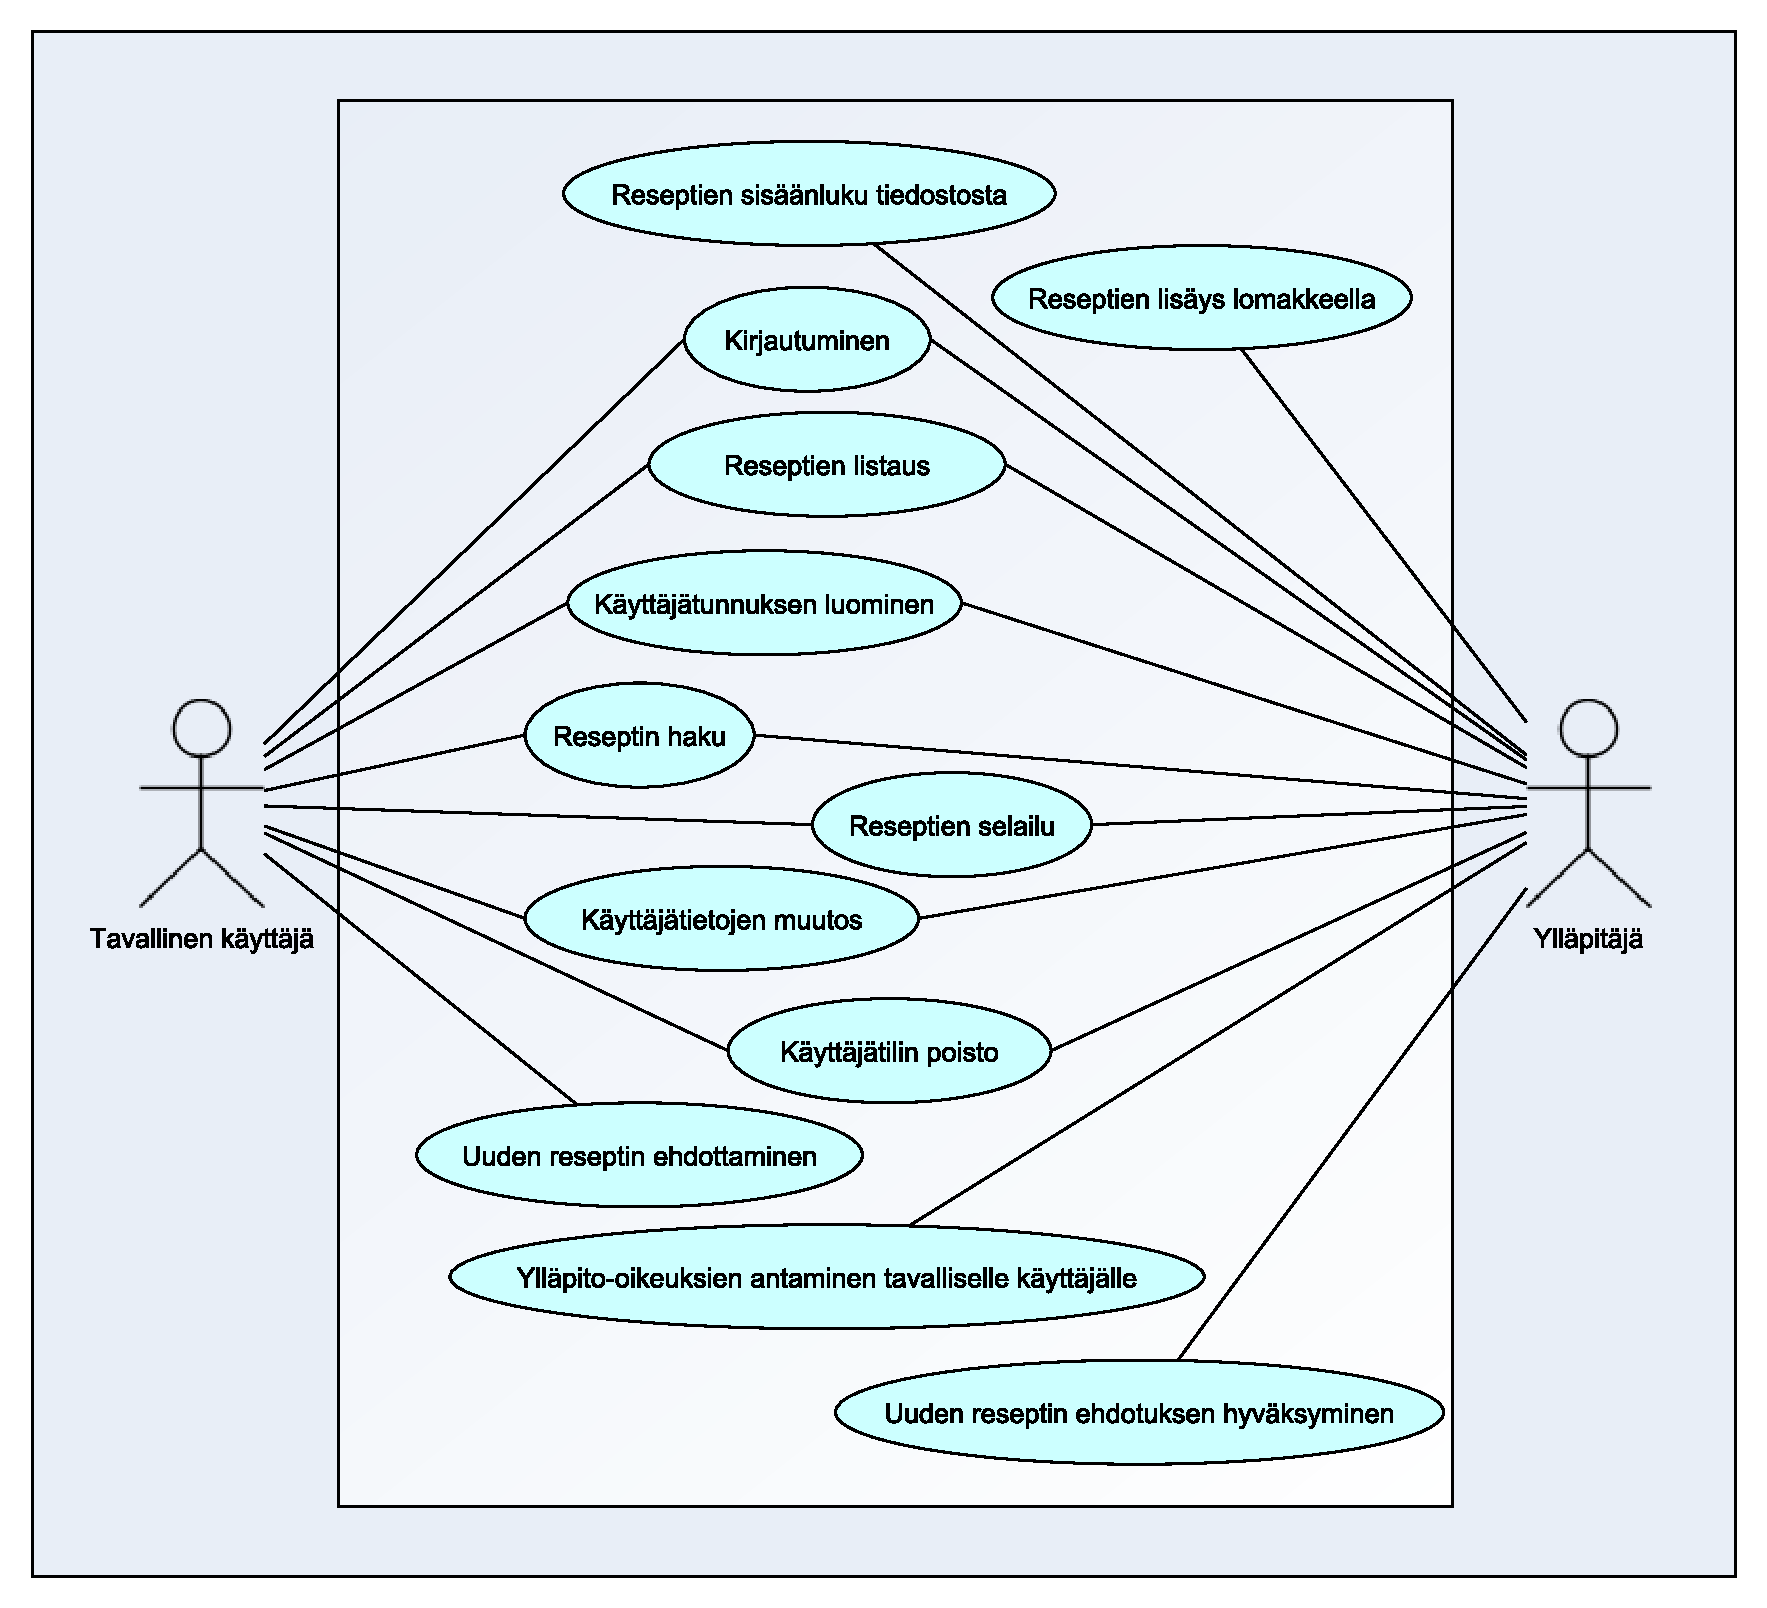
\includegraphics[scale=0.4]{kayttotapaukset.pdf}.
\\*
\subsection{Käyttäjäryhmät}

\begin{flushleft}Ylläpitäjä\end{flushleft}

Ylläpitäjän pitää olla rekisteröitynyt lomakkeen käyttäjä, jolle on annettu ylläpito-oikeudet. Lomake vaatii sisäänkirjautumisen.

\begin{flushleft}Tavallinen käyttäjä\end{flushleft}

Tavallinen käyttäjä voi olla kuka tahansa sivulle kirjautunut henkilö. 

\subsection{Käyttötapaukset}

\begin{flushleft}\textbf{Ylläpitäjä\(\colon\)} \end{flushleft}

Reseptien haku\(\colon\) käyttäjä voi hakea tietokannasta reseptejä hakusanalla. Yksi hakusana voi tuottaa monta tulosta.

Reseptien listaus\(\colon\) käyttäjä voi listata reseptit ainesosan mukaan tai aakkos-- tai juomalajijärjestykseen.

Ylläpito-oikeuden antaminen tavalliselle käyttäjälle\(\colon\) käyttäjä voi tehdä tavallisesta käyttäjästä ylläpitäjän. 

Uuden reseptin ehdotuksen hyväksyminen\(\colon\) käyttäjä voi hyväksyä tavallisen käyttäjän reseptiehdotuksen, ja lisätä reseptin tietokantaan.

Reseptin lisäys lomakkeella\(\colon\) käyttäjä voi lisätä reseptin käyttäen siihen tarkoitettua lomaketta.

Reseptin lisäys tiedostosta\(\colon\) käyttäjä voi lisätä uuden reseptin lukemalla sen suoraan tiedostosta. 

Muut käyttötapaukset\(\colon\) Käyttäjätietojen muutos, käyttäjätilin poisto, käyttäjätunnuksen luominen, reseptien selaaminen, kirjautuminen

\begin{flushleft}\textbf{Tavallinen käyttäjä\(\colon\)}\end{flushleft}

Reseptien haku\(\colon\) käyttäjä voi hakea tietokannasta reseptejä hakusanalla. Yksi hakusana voi tuottaa monta tulosta.

Reseptien listaus\(\colon\) käyttäjä voi listata reseptit ainesosan mukaan tai aakkos-- tai juomalajijärjestykseen.

Uuden reseptin ehdottaminen\(\colon\) käyttäjä voi ehdottaa uutta reseptiä ylläpitäjälle lisättäväksi tietokantaan.
 
Muut käyttötapaukset\(\colon\) Käyttäjätietojen muutos, käyttäjätilin poisto, käyttäjätunnuksen luominen, reseptien selaaminen, kirjautuminen

\end{document}